\section{W04 - Process Design}
 
\subsection{Process Design}
\subsubsection{Definition: (Process)Design}
\index{Design!Definition}
\begin{itemize}
\item To design is to conceive the looks, arrangement, and
workings \textbf{before} something is constructed
\item Design is therefore a \textbf{conceptual activity} that has to
deliver a solution that works in practice
\item In some languages ''design'' has a stronger connotation
with the looks of an object (artistic aspects)
\end{itemize}
\subsubsection{Designer’s Aims}
\begin{tabular}{|p{7cm}|p{7cm}|}
	\hline Product designers will seek to create things that... &  Operation managers tend to focus on the design of the tranformation process- which..\\ 
	\hline  
	are aesthetically pleasing& is flexible and efficient \\ 
	satisfy needs& supports the stategic goals of companies \\ 
	meet expcetations& is without errors \\ 
	perform well& is motivating for employees \\ 
	are reliable& is robust and easy to control \\ 
	are easy to manufacture and deliver	&  \\ 
	\hline 
\end{tabular} 
\subsubsection{Relationship between Product and Process Design}
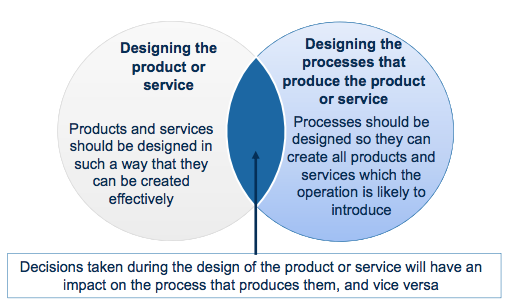
\includegraphics[width=1\textwidth]{W04/product_process_design}
\subsection{Process Types}
\subsubsection{Manufacturing Process Types\index{Process Types}}

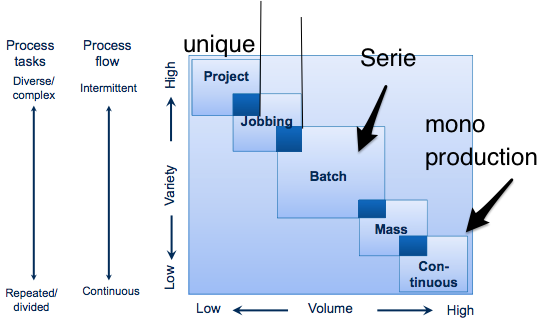
\includegraphics[width=1\textwidth]{W04/manufacturingprocesstype}
\subsubsection{Project Processes \index{Project Processes}}
\begin{itemize}
\item One-off, complex, large-scale 'products' with a
high work content
\item Defined start and finish: time, quality, and cost
objectives
\item Specially made, every one 'customized'
(engineered to order)
\item Complex planning, as many different skills have
to be coordinated
\item Fixed position layout: material is assigned to the
object
\item Examples: \textbf{Construction site}, shipyard, plant
construction
\end{itemize}
\subsubsection{Jobbing Processes\index{Jobbing Processes}}
\begin{itemize}
\item Very small quantities: 'one-offs', or only a few
required
\item Specially made: every one 'customized'
(make to order)
\item High variety and low repetition
\item Skill requirements are usually very broad
\item Skilled jobbers or team complete whole
product
\item Fixed position or functional layout
\item Examples: \textbf{Machine industry}, press cylinder,
tailor-made suits
\end{itemize}
\subsubsection{Batch Processes\index{Batch Processes}}
\begin{itemize}
\item Higher volumes and lower variety than
for jobbing
\item Standard products, repeating demand
(but can be made to order)
\item Specialized, narrower skills
\item Set-ups (changeovers) at each stage of
production
\item Functional or cell layout
\item Example: Machine tool manufacturing,
food production, clothing,\textbf{ canteen
kitchen}
\end{itemize}
50x Los am Tag produzieren / B\"acker Batch(Teig) zu Brot verarbeiten
\subsubsection{Mass Processes\index{Mass Processes}}
\begin{itemize}
\item Higher volumes than batch
\item Standard, repeat products (make to
stock) or with customer-specific
assembly (mass customization)
\item Low and/or narrow skills; high degree
of work split
\item No change-overs, or almost
instantaneous ones
\item Cell or product layout
\item Example: Automotive production,
mass electronics,\textbf{ beer bottling}
\end{itemize}
Tages-/Wochenarbeit, Automatisiert, Fluss steht im Zentrum, wenn ein Anlageteil steht so steht die ganze Produktion.
\subsubsection{Continuous Processes\index{Continuous Processes}}
\begin{itemize}
\item Extremely high volumes and low
variety:
often single product in endless flow
\item Standard, repeat products (make to
stock)
\item Highly capital-intensive and automated
\item Few change-overs required
\item Difficult and expensive to start and stop
the process, therefore few changeovers
\item Example: \textbf{petrochemical refineries},
steel-making industry, internet server
\end{itemize}

\subsubsection{\index{Process!Types}Process Types: Services }
\subsubsection{Costs of Operations}
Bsp: Beratung, wird nicht schneller mit n-Personen mehr.\\
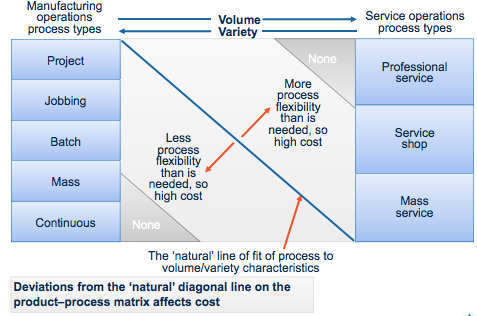
\includegraphics[width=1\textwidth]{W04/costofoperations}
\newpage
\subsection{Methods and Tools}
\subsubsection{\index{Little's Law}Little\textquotesingle{}s Law - Example }
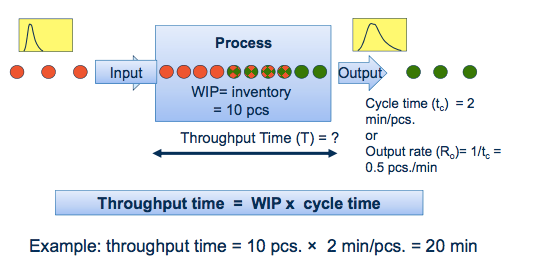
\includegraphics[width=1\textwidth]{W04/littleslaw}
\subsubsection{Little\textquotesingle{}s Law\index{Little's Law}}\label{littleslaw}
\begin{center}
	Alles in der Blackbox, egal ob in Warteschlange oder Nacharbeit, wird als Work in Progress (WIP) gez\"ahlt\\
	\begin{tabular}{|r|c|l|}
	\hline T  & Troughput time & s/min/h \\ 
	\hline WIP & Work in Progress & piece/kg/CHF \\ 
	\hline $t_c$ & cycle time & time per piece\\ 
	\hline $R_0$ & Output rate & $\frac{piece}{time}$\\
	\hline
\end{tabular}
\\\vspace{5 mm}

	$R_0$ = $\frac{1}{t_c}$ \\\vspace{2 mm}
	T =$ WIP\cdot cycle time$ \\\vspace{2 mm}
	T = $\frac{WIP}{output rate}$\\\vspace{2 mm}

\end{center}
\subsubsection{Example: Snowboarding}
\begin{center}
	120 Snowboarders ar waiting, everey 8 seconds 4 where transported.\\\vspace{2 mm}
$WIP = 120 SB $\\\vspace{2 mm}
$t_c = \frac{8 [sec]}{4[SB]} = 2[sec/SB]$ \\\vspace{2 mm}
$T = 120 [SB] \cdot 2[t_c] = 240 [sec] = 4 [min] $ \\\vspace{2 mm}
\end{center}
\subsubsection{Throughput time\index{Throughput!Time} and Processing Time\index{Processing!Time} Are not the Same!}
Nur Bearbeitungszeit ist wertsch\"opfend, Transportzeit kann auch wertsch|"opfend sein.\\
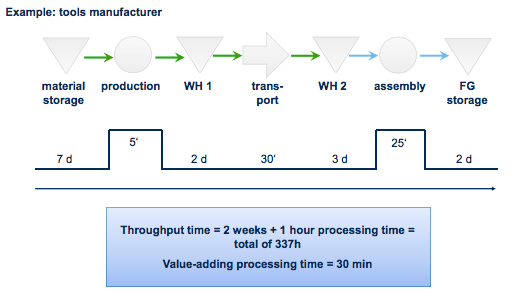
\includegraphics[width=1\textwidth]{W04/troughputvsprocessing}
\subsubsection{Little's Law Exercise: Automotive Supply Chain\index{Little’s Law}}
\begin{itemize}
\item An automotive OEM produces a new car every 2
minutes. The throughput time (from arrival of raw
materials until the car is ready for distribution) is 2
weeks. Please calculate the capital tied up in the
OEMs supply chain
\item Average value of the car during the 2 weeks of
production: CHF 20,000
\item Manufacturer's working time: 3 x 8-hour shifts on 5
days a week
\end{itemize}
\begin{center}
	
$Gebundenes Kapital minimieren \Longrightarrow schneller arbeiten$\\
$t_c = 2min =\frac{1}{30}h$\\
$T = 2w \cdot 5d \cdot 3 shifts = 240h$\\
$Bestand = 7200 Cars \cdot 20'000 = 144'000'000$\\ \vspace{2mm}
$20'000 \cdot \frac{2 \cdot 5 \cdot 24 \cdot 60}{2}=144'000'000$
\end{center}
\subsubsection{Division of Labor - Example\index{Division of Labor}}
\begin{center}
\begin{tabular}{|c|c|c|c|}
\hline Code & Activity & Predecessor & Time (min)\\ 
\hline A & Pretest  1&  - & 5\\ 
\hline B & Pretest 2 & A & 6\\ 
\hline C & De-assembly & B & 4\\ 
\hline D & Repair 1 & C & 8\\ 
\hline E & Repair 2 & C & 6\\ 
\hline F & Repair 3 & C & 4\\ 
\hline G & Assembly & D, E, F & 10\\ 
\hline
\end{tabular} 
\end{center} 
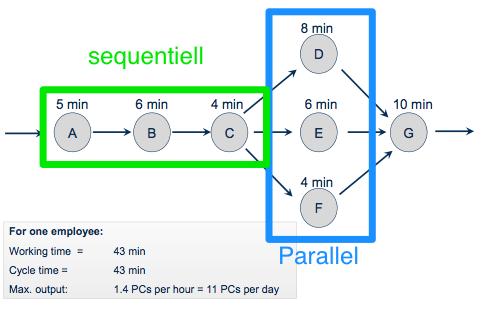
\includegraphics[width=1\textwidth]{W04/processmap}
\index{Parallel}
\index{Sequentiell}
\index{Process!Map}
\subsubsection{Division of Labor\index{Division of Labor}}
L\"angster Schritt diktiert denn Takt. \index{Balancing!Loss}Balancing Loss weil wartezeit pro Zyklus anf\"allt.\\
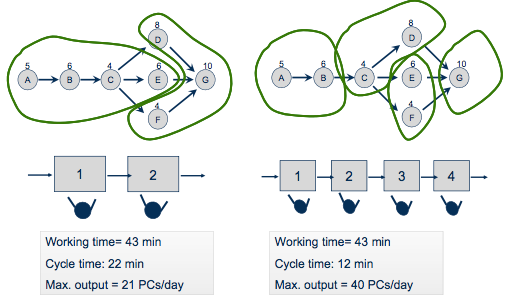
\includegraphics[width=1\textwidth]{W04/divisionoflabor}
\subsubsection{In Series (Sequentially\index{Sequentially}) or in Parallel\index{Parallel}?}
\begin{tabular}{|>{\centering\arraybackslash}p{7cm}|>{\centering\arraybackslash}p{7cm}|}
	\hline serie & parallel \\ 
	\hline kosteneffizient & robust (Ausfall) \\ 
	Erfahrungskurve (20-30\%) & flexibel(Volumen)\\
	 Weniger Platz (Infrastruktur $\cdot1$)& Variantenvielfalt
	 \\ Produktequalit\"at &   Servicequalit\"at\\ 
	\hline 
	Channeled flow, easier to manage & Higher mix flexibility \\
	Simple material handling & Higher volumen flexiblity \\
	Lower capital requirements & Higher robustness\\
	More efficient operation (higher propotion of direct productive work) & Less monotony[1]
\\
Space-saving & Greater autononmy[1] \\
	\hline
\end{tabular} 
[1] Employee motivation\\
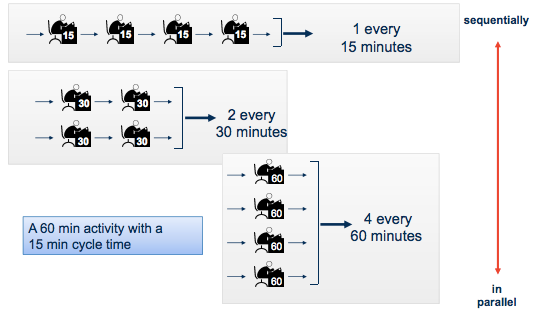
\includegraphics[width=1\textwidth]{W04/sqvspar}

\subsubsection{Balancing Processes to Avoid Loss of Efficiency}
\index{Balancing!Loss}
Verlustzeit aufgrund Arbeitsteilung, je mehr sequentiell desto h\"oher Balance Loss (Achtung Lernkurve).\\
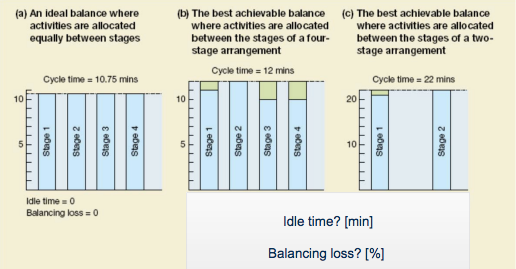
\includegraphics[width=1\textwidth]{W04/balancingprocess}